\documentclass[11pt]{article}  %11 or 12 pt

\usepackage{graphics,graphicx}
\usepackage{color, colortbl}
\usepackage{multicol} 
\usepackage{parskip}
\usepackage{amsmath}
\usepackage{multirow}
\usepackage[utf8]{inputenc}
\usepackage{fancyhdr}
\usepackage[title]{appendix}
\usepackage{wasysym}
\usepackage{url}
\usepackage{subcaption}

\usepackage[font=footnotesize,labelfont=small]{caption}
\captionsetup{width=0.85\linewidth}
\definecolor{LightCyan}{rgb}{0.7,1,1}

\RequirePackage{geometry}
\geometry{margin=0.65in}

\renewcommand{\rmdefault}{phv} % Arial
\renewcommand{\sfdefault}{phv} % Arial

\usepackage{sectsty} % can change font, size of the section headings.  
\sectionfont      {\fontsize{12pt}{3}\usefont{OT1}{phv}{b}{sc}\selectfont}
\subsectionfont   {\fontsize{11pt}{3}\usefont{OT1}{phv}{b}{n}\selectfont}
\subsubsectionfont{\fontsize{11pt}{3}\usefont{OT1}{phv}{m}{n}\selectfont}

\renewcommand{\thesection}{\Alph{section}} % so that section headings use A B C instead 1 2 3
\renewcommand{\baselinestretch}{1}

\newcommand{\inden}[1]{\mbox{} \hspace{#1} } % Force horizontal spaces.  

\setlength{\parskip}{0.2cm}
\setlength{\parindent}{0pt}
\renewcommand{\baselinestretch}{1.15}

\title{Spiking Neural Network on \\ Gender Classification from Speech Data}
\author{
	Tai D. Nguyen,  Adarsha Baiji, Anup K. Das\\
	Dept. Electrical and Computer Engineering \\
	Drexel University \\
	Philadelphia, PA, USA \\
	\{tdn47, ab3586, ad3639\}@drexel.edu
}
\date{\today}

\begin{document}

\maketitle

\begin{abstract}
 Spiking Neural Network, or SNN, provides a good trade-off between power consumption and accuracy, in comparison to a Convolutional Neural Network (CNN) of the same size. In an SNN, only a portion of the connected neurons remains active to fire spikes in a particular fashion, when the network is presented with a stimulus at the input layer. This behavior allows the network to not only be very energy efficient but also be capable of employing biologically plausible plasticity rules. In this paper, two SNN models, unsupervised and supervised are simulated using C++ and applied to classify gender information in speech data. Our models are able to achieve an accuracy of 78.85\% and 90.05\%, while consuming 232 and 35 times less power, respectively, in comparison to a CNN of the same size.
\end{abstract}

\section{Introduction}
\label{intro}

It is no myths that Convolutional Neural Network and its derivates are computationally intensive \cite{b1}. Hence, no meaningful machine learning applications using CNNs can be run on ultra-low energy, microelectronic devices in a reasonable amount of time. Often, data from customers' sensors are collected and sent to a powerful super-computer for processing. However, this is not how human brains work -- we do not amass gigabytes of information from every sensor in our body every millisecond and send it somewhere for processing. We would drive into each other before we can react to the things in front of our eyes. Therefore, in order to advance the state of art in the field of human-machine integration, it is necessary to introduce machine learning capabilities with good classification accuracy and security into ultra-low energy microelectronics. If this is achievable, it is possible for humans and machines to integrate using Brain-Machine Interfaces (BMI), currently developed by researchers at Neuralink \cite{b2}. In this paper, Spiking Neural Networks will be shown that they can be the solution to the predicaments of information processing in machine-human integration. 

\section{Background on Spiking Neural Network}
\label{bg_snn}

\subsection{Spiking Neural Network}

Spiking Neural Networks are fundamentally different from any second generation's neural nets. Their neuronal models operate closely to those inside the human brain. In short, two neurons, the pre-synaptic neuron, and the post-synaptic neuron are connected by a synapse with a certain \textit{weight number}. As the pre-synaptic neuron fires spikes towards the post-synaptic neuron, electrical charges accumulate at the latter until its potential threshold is breached. Once breached, the neuron sends spikes towards the next neuron it is connected to, and its membrane potential is reset \cite{b3}. Using this neuronal behavior, the network "learns" using Spike-Timing Dependent Plasticity (STDP), which is a principle that partially explains the biological process of synapses' strength adjustments. STDP states that \cite{b4}:

\begin{itemize}
	\item Long-term potentiation (LTP) occurs when the pre-synaptic neuron spikes immediately \textit{before} the post-synaptic neuron spikes.
	\item Long-term depression (LTD) occures when the pre-synaptic neuron spikes immediately \textit{after} the post-synaptic neuron spikes.
\end{itemize}

Hence, in our SNN neuron model, the \textit{weight number}, which determines the likelihood of the pre-synaptic neuron to spike the next time around, increases with LTP and decreases with LTD. In a network trained with STDP, a certain group of neurons will fire in a certain pattern when a particular stimulus is introduced at the input layer. 

\begin{figure}[!htb]
	\centering
	\includegraphics[width=0.6\linewidth]{"neuron model"}
	\caption{Simplified Spiking Neuron Model}
	\label{fig:neuron-model}
\end{figure}


\subsection{Leaky Integrate-and-Fire Neurons}

There are 3 common neuronal models (listed with increasing complexity): Leaky Integrate-and-Fire (LIF), Izhikevic 4-parameters, and Izhikevic 9-parameters. This paper will focus only on the LIF model, whose neurons' behavior is governed by the following equation \cite{b5}:

\begin{equation}
	C\frac{dV}{dt} = -g_L(V(t) - V_R) + I(t)
	\label{eq1}
\end{equation}

A LIF neuron is a parallel combination of a "leaky" resistor with conductance $g_L$ and a capacitor with capacitance $C$. When $V(t)$ reaches a threshold level $V_{th}$, the capacitor discharges to a resting potential $V_R$. Since the biological neuron also "undershoots" $V_R$ at the discharging phase (so-called Afterhyperpolarization - AHP), there exists a relative refractory period where the neuron cannot fire any new spikes if it is depolarized by smaller or equal potential. This behavior can be modeled with a dynamic potential threshold $V_{th}$: following each spike, increase $V_{th}$ by a small amount \cite{b6}:

\begin{equation}
	V_{th\_next} = V_{th\_prev}(1+\tau t)
	\label{eq2}
\end{equation}

where $t$ is the amount of time passed from last spike. 

\subsection{Poisson Spike Model}

One problem with the LIF neuron model described above is that it is too deterministic in comparison to neurons in the cortex. The spikes generated by our brains' neurons are highly randomized, which insinuates two possible theories:

\begin{itemize}
	\item Theory 1: The irregular interspike interval (ISI) represents a random process, where the exact moments of the spikes do not hold meaningful information, but rather facilitate noise introduction into the system.
	\item Theory 2: The spike timing holds relevant information about a pre-synaptic event. Hence the ISI in conjunction with firing rate can represents a very large amount of information.
\end{itemize}

From these two theories, there are two main information encoding techniques: rate encoding and time encoding. Rate encoding is done by translating information into the number of spikes per unit time; and time encoding is accomplished by converting information into ISI. The SNN described in this paper leverages rate encoding together with a Poisson Spike model to preserve the property of "randomness".

The equation describing Poisson distribution is known as:

\begin{equation}
	f(k; \lambda) = \frac{\lambda^k e^{-k}}{k!}
	\label{eq3}
\end{equation}

Hence, if the spike rate $r$ is defined as the number of spikes $s$ over an interval $T$, $r = s/T$, then the probability that $n$ spikes ($n < s$) happen in a sub-interval $\Delta t$ is:
	
\begin{equation}
	P(n \in \Delta t) = C^n_s(\Delta t/T)^n(1- \Delta t/T)^{s-n}
	\label{eq4}
\end{equation}

if $k \rightarrow \infty$, $T \rightarrow \infty$ and $r$ stays constant:

\begin{equation}
	P(n \in \Delta t) = \frac{(r\Delta t)^n e^{-r\Delta t}}{n!}
	\label{eq5}
\end{equation}

When $\Delta t$ is small and $r\Delta t << 1$, $P(n=1 \in \Delta t)$ can be approximated with $r\Delta t$. Hence, for each interval $i$, a number between 0 and 1 is generated from the Uniform distribution, $x[i]$, such that: if $x[i] \le r\Delta t$, then a spike is initiated. The SNN described here uses this method to encode audio information into spike trains.

\section{Background on CARLsim4}
\label{bg_carlsim4}

As a collaborative effort between Drexel University (DU) and the University of California, Irvine (UCI) to advance in the domain of Spiking Neural Networks, the SNN simulator chosen for this paper is CARLsim4. 

CARLsim4 is a GPU-accelerated SNN simulation tool written in C++ by researchers at the Cognitive Anteater Robotics Laboratory in UCI. This software provides the basic underlying framework to create an application using a Spiking Neural Network. Its discovered and understood capabilities \footnote{Other capabilities are available in the software but will not be focused.} include:

\begin{itemize}
	\item Definitions of the Izhikevich 4-Parameters, Izhikevich 9-Parameters, and LIF neuronal model
	\item Mechanisms to support building connections between groups of neurons of the same/different model
	\item Mechanisms to support simulating information encoding and spike train generation 
	\item Mechanisms to support STDP and Homeostasis
	\item Two monitoring mechanisms for developing and post-processing
	\item GPU accelerated for very large networks
\end{itemize}

CARLsim4's workflow composes of 3 states: Config, Setup, and Run. The Config state is where the topologies of the network, or, groups of neurons along with their connections to one another are defined. The Setup state allows the user to choose the back-end (CPU or GPU) of the network, and bring up monitors to look at a particular neuron/layer. The Run state is responsible for spike train generation and the executions of all neurons in the network. The state/output of the network can also be stored for post-processing or demoing at the end of the Run state.

Also, two monitoring tools, available in CALRsim4, can write outputs to binary files, which can be used in the software's MATLAB Offline Analysis Toolbox (OAT). The outputs of the SNN in this paper will be piped into MATLAB for K-Means clustering.

\section{Background on DARPA's TIMIT Acoustic-Phonetic Continuous Speech Dataset}
\label{dataset}

This dataset (will be referred later on as TIMIT) is created as a joint effort between Massachusetts Institute of Technology (MIT), Stanford Research Institute (SRI), and Texas Instruments (TI), under the funding of the Defense Advanced Research Projects Agency - Information Science and Technology Office (DARPA-ISTO) \cite{b7}. 

TIMIT contains the transcripts and CD-quality audio data of 6300 sentences, in which the same 10 sentences are recorded by each of the 630 speakers from 8 major dialects in the United States of America. The dialects' regions are as follows:

\begin{itemize}
	\item DR1: New England
	\item DR2: Northern
	\item DR3: North Midland
	\item DR4: South Midland
	\item DR5: Southern
	\item DR6: New York City
	\item DR7: Western
	\item DR8: Army Brat (moved around)
\end{itemize}

The gender distribution for each region is listed in Table \ref{table1} below:

\begin{table}[htbp]
	\begin{center}
		\begin{tabular}{|c|c|c|c|}
			\hline
			\textbf{Dialect Region (DR)}&\textbf{\# Male}&\textbf{\# Female}&\textbf{Total} \\
			\hline
			1 & 31 (63\%) & 18 (27\%) & 49 (8\%) \\
			\hline
			2 & 71 (70\%) & 31 (30\%) & 102 (16\%) \\
			\hline
			3 & 79 (67\%) & 23 (23\%) & 102 (16\%) \\
			\hline
			4 & 69 (69\%) & 31 (31\%) & 100 (16\%) \\
			\hline
			5 & 62 (63\%) & 36 (37\%) & 98 (16\%) \\
			\hline
			6 & 30 (65\%) & 16 (35\%) & 46 (7\%) \\
			\hline
			7 & 74 (74\%) & 26 (26\%) & 100 (16\%) \\
			\hline
			8 & 22 (67\%) & 11 (33\%) & 33 (5\%) \\
			\hline
			\rowcolor{LightCyan}
			ALL & 438 (70\%) & 192 (30\%) & 630 (100\%) \\
			\hline
		\end{tabular}
		\caption{Table detailing the gender distribution for each dialect region in TIMIT}
		\label{table1}
	\end{center}
\end{table}

From the table above, it is clear that TIMIT is skewed because the male population is 2.3 times the female population. Hence, for balancing, speech data from 192 randomly selected males (out of 438) will be chosen to form the database along with those from 192 females. Therefore, the total amount of audio clips to be processed is 3840.

\section{Experimental Setup}
\label{experimental_setup}

\subsection{Data Pre-processing Using MFCCs}

% Include a flow diagram of the data preprocessing steps
\begin{figure}[!htb]
	\centering
	\includegraphics[width=0.6\linewidth]{"data preprocessing"}
	\caption{Flow diagram of the data pre-processing process}
	\label{fig:data-preprocessing}
\end{figure}


The audio data available is in the "wav" file format -- a list of millions of 32-bit floating point numbers. There are no correlations between these numbers and the speaker's gender. Hence, it is necessary to transform the data into a different, more concise and more meaningful representation. The most famous transformation is the Short-Term-Fourier-Transform (STFT), which produces a spectrogram -- a 2D matrix that entails the energy at a certain frequency band in a particular time period. 

Since the dataset is composed of people with diverse dialects speaking distinct sentences, the STFT spectrogram will look tremendously different from person to person and from sentences to sentences. Therefore, in order to further concise the STFT spectrogram to eliminate these differences, a spectrogram-of-a-spectrogram, or, a cepstral is constructed for each audio signal. In addition, the filter banks (frequency bands) used in the first spectrogram is derived from the nonlinear Mel scale \cite{b8} so that the resulting spectra reflect human hearing better. This combination is called the Mel-frequency cepstrum (MFC). And the coefficients of all MFCs are called the Mel-frequency cepstral coefficients (MFCC).

% Insert figure of STFT spectrogram vs Mel spectrogram
\begin{figure}[htb!]
	\centering
	\begin{subfigure}[b]{.4\linewidth}
		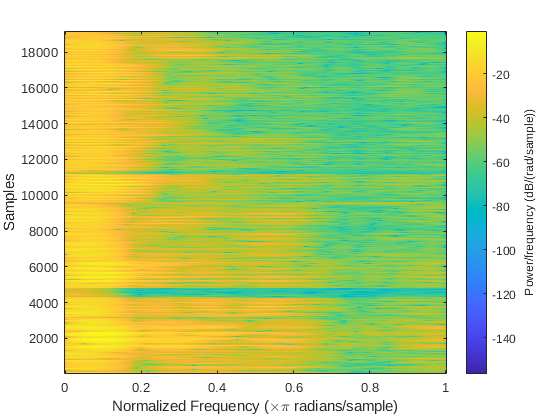
\includegraphics[width=\textwidth]{stft1.png}
		\caption{STFT Spectrogram of speaker 1 sentence 1}
		\label{fig:stft-speaker1-sent-1}
	\end{subfigure}
	%	\hskip2em
	\begin{subfigure}[b]{.4\linewidth}
		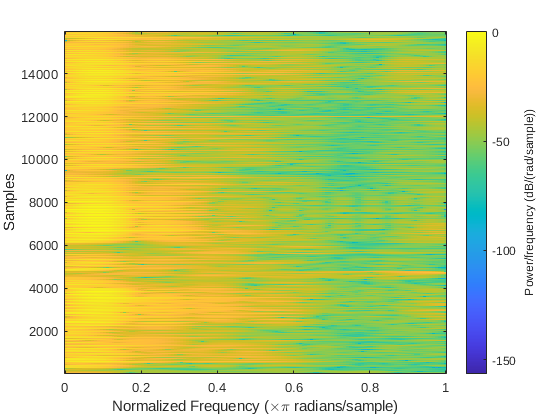
\includegraphics[width=\textwidth]{stft2.png}
		\caption{STFT Spectrogram of speaker 1 sentence 2}
		\label{fig:stft-speaker1-sent-2}
	\end{subfigure}

	\begin{subfigure}[b]{.4\linewidth}
	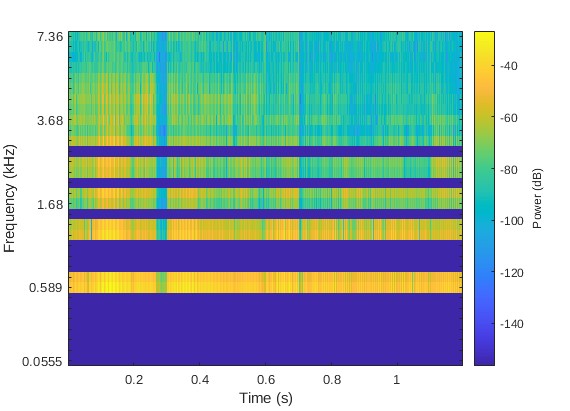
\includegraphics[width=\textwidth]{mel1.png}
	\caption{Mel Spectrogram of speaker 1 sentence 1}
	\label{fig:mel-speaker1-sent-1}
	\end{subfigure}
	%	\hskip2em
	\begin{subfigure}[b]{.4\linewidth}
		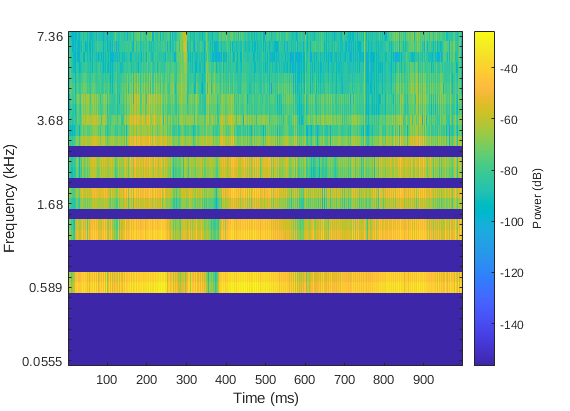
\includegraphics[width=\textwidth]{mel2.png}
		\caption{Mel Spectrogram of speaker 1 sentence 2}
		\label{fig:mel-speaker1-sent-2}
	\end{subfigure}
	\caption{Top (a,b): STFT Spectrograms of speaker 1 with 2 different sentences. Bottom (c,d): Mel Spectrograms of the same speaker with the same 2 sentences. It is clear that the STFT Spectrogram provides too much information with respect to individual audio signal, while the Mel Spectrogram provides much more compact information, which is useful in determining gender from speech}
\end{figure}

As audio signals in the database have different lengths, to make all Mel spectrograms congruent in shape for the neural network, different window lengths \footnote{with overlap length equals to half of window length} (in number of samples) are calculated for each signal so that the number of windows for the entire signal is always 99 ($50\times 2-1$).

In addition to performing MFCC analysis on each audio signal, silent and noise removal is also performed before doing MFCC to further increase the ratio of relevant to irrelevant information in the output signal.

\subsection{SNN Architecture}

% Insert figure of the SNN Architecture
\begin{figure}[!htb]
	\centering
	\includegraphics[width=0.6\linewidth]{"snn topology"}
	\caption{The topology of the Spiking Neural Network}
	\label{fig:snn-topology}
\end{figure}

The pre-processed audio signals are fed into the SNN one by one. Since the size of the MFCC is 13 by 99, the input layer will have 1287 neurons -- one neuron for every coefficient. In the second layer, every neuron is connected to 3 neurons in the previous layer in a 1 by 3 kernel with a stride of 1 in the x-direction and 3 in the y-direction. These non-overlapping connections are meant to discover patterns in each of the small region of the MFCC. The third layer is connected to the second layer the same way the second layer is connected to the input layer. However, the type of neurons in this layer is \textbf{\textit{max-pooling}} instead of LIF. 

A \textit{\textbf{max-pooling}} spiking neuron must connect with more than one neurons from the previous layer. Out of all the connected neurons, it will detect and transfer the spike train of the one with higher activity. The activity of a neuron is defined as the number of spikes emitted in a period of time. 

The output of the max-pooling layer will be used for post-processing. The unsupervised version of this architecture uses k-means clustering. The supervised version, however, uses k-nearest-neighbor for training and classification. 

\section{Simulation Results}
\label{sim_res}

\subsection{Accuracy Rating}

For the unsupervised architecture, applying k-means on the SNN's output over 500 iterations give: 
\begin{itemize}
	\item The highest accuracy reported is 80.53\%
	\item The lowest accuracy reported is 77.83\%
\end{itemize}


With regards to the supervised architecture, which performed k-nearest-neighbors (with the cityblock distance function and $k=20$) on the SNN's output:
\begin{itemize}
	\item The accuracy obtained for the training set of 2880 audio clips (75\%) is 89.05\%
	\item The accuracy obtained for the testing set of 960 audio clips (25\%) is 90.05\%
\end{itemize}


If instead of KNN, a Support Vector Machine (box constraint = 0.05, kernel function = linear, kernel scale = 2) is used for classification at the output of the SNN, then the ratings are:
\begin{itemize}
	\item The accuracy obtained for the training set of 2880 audio clips (75\%) is 91.56\%
	\item The accuracy obtained for the testing set of 960 audio clips (25\%) is 92.30\%
\end{itemize}

Using MATLAB's Deep Learning Toolbox, a Convolutional Neural Network is created with similar architecture as the SNN:

\begin{itemize}
	\item Input layer of 13 by 99
	\item Convolutional 2D layer with kernel 1 by 3, x-stride of 1 and y-stride of 3
	\item A Batch Normalization Layer
	\item A ReLU activation layer
	\item A Softmax Layer
	\item A Classification Layer (0 for male, 1 for female)
\end{itemize}

The network performance has high variance. The highest recorded accuracy is 89.90\% and the lowest is 67.08\%.

% Insert graph of accuracy ratings
\begin{figure}
	\centering
	\includegraphics[width=0.7\linewidth]{"accuracy rating"}
	\caption{}
	\label{fig:accuracy-rating}
\end{figure}


\subsection{Energy and Speed Rating}

The energy rating shown below is an estimation of the total amount of energy (in Joules) for the different architectures in the sub-section above. With respect to the SNN, the recorded total number of spikes is 178,357,388. For each spikes, the amount of energy needed is 35 pJ \cite{b9}, where the overhead of the neuron in a neuromorphic device is accounted for. Hence, the total amount of energy consumed by the SNN is: \textbf{6.24 mJ}.

Regarding the three algorithms: k-means, KNN, and SVM, their execution times \footnote{averaged over 100 runs} are used to estimate their energy rating. The host system's CPU is an Intel Core i5-7300HQ, which has an energy consumption of about 45W for 4 cores (11.25W/core) \footnote{assuming all cores have equal energy consumption}, each with a maximum clock frequency of 3.5GHz. Hence, if all algorithms are forced to utilize 100\% of all resources available on one core, the energy consumptions for each algorithm is:
\begin{equation}
	E = T \times \frac{45J}{s} \times \frac{1}{\text{4 cores}}
\end{equation}

where E is energy (J), and T is execution time (seconds)

% Insert table of energy rating
\begin{table}[htbp]
	\begin{center}
		\begin{tabular}{|c|c|c|c|}
			\hline
			\textbf{Algorithm}&\textbf{Execution Time (s)}&\textbf{Energy Consumption (mJ)}&\textbf{Energy Consumption with SNN (mJ)} \\
			\hline
			K-means & 0.0295 & 332.3 & 338.5 \\
			\hline
			KNN & 0.1990 & 2239.5 & 2245.7 \\
			\hline
			SVM & 0.3060 & 3443.3 & 3449.5 \\
			\hline
		\end{tabular}
		\caption{Table detailing energy consumptions in Joules between K-means, KNN, and SVM}
		\label{table2}
	\end{center}
\end{table}

%\newpage

Using the same host-system setup and the same method of rating energy consumption, the CNN shown in the previous section runs for 10 epochs -- the average total runtime (over 20 trials) of \textbf{6.9876 seconds}. Hence, its energy consumption is: 78610.5 mJ, which is \textbf{232, 35, 23} times the amount of energy needed to run SNN + K-means, SNN + KNN, and SNN + SVM, respectively.

\section{Conclusions and Future Works}
\label{future_works}

It is clear that SNN provides a clear advantage over CNN (of the same size) when it comes to power efficiency because:
\begin{itemize}
	\item Only a number of neurons are active at any given time in an SNN
	\item Spikes are either there or not there at any given time. Hence, no floating-point operations needed
	\item The implementation of neurons and spikes in neuromorphic hardware allows for many energy/heat optimization
\end{itemize}

Regarding accuracy ratings, the hybrid SNN architectures result in good classification performance with respect to other types of networks of similar complexity. There are many optimizations in the spiking domain which are being developed in CARLsim4 by our team at the Distributed Intelligent Scalable Computing Lab (DISCO) at Drexel University. Some are listed here, but not restricted to:

\begin{itemize}
	\item Adaptive neuronal parameters
	\item Weight and threshold balancing to reduce noise in the network
	\item More controllable rate of spiking so that neurons only fires when it has substantial information
	\item Better encoding techniques (i.e, a hybrid between rate and time encoding)
	\item Introduction of "hint" network -- a secondary network that is responsible for learning patterns within the main network itself so as to drive the main network to converge faster (in supervised learning)
	\item Optimization of the delay in spike traveling signals on neuromorphic devices
\end{itemize}

\newpage

\begin{thebibliography}{00}
	\bibitem{b1} Hyunbin Park, Dohyun Kim and Shiho Kim.
	\newblock Digital Neuron: A Hardware Inference Accelerator for Convolutional Deep Neural Networks, 2018;
	\newblock arXiv:1812.07517.
	\bibitem{b2} Musk, Elon. “An Integrated Brain-Machine Interface Platform with Thousands of Channels.” 2019, doi:10.1101/703801.
	\bibitem{b3} Koch, Christof; Segev, Idan (1999). Methods in neuronal modeling : from ions to networks (2nd ed.). Cambridge, Massachusetts: MIT Press. p. 687. ISBN 978-0-262-11231-4
	\bibitem{b4} Gilson, Matthieu. “STDP in Recurrent Neuronal Networks.” Frontiers in Computational Neuroscience, vol. 4, 2010, doi:10.3389/fncom.2010.00023.
	\bibitem{b5} Teeter, Corinne, et al. “Generalized Leaky Integrate-and-Fire Models Classify Multiple Neuron Types.” Nature Communications, vol. 9, no. 1, 2018, doi:10.1038/s41467-017-02717-4.
	\bibitem{b6} D.C.Somers, S.B.Nelson, and M.Sur. An emergent model of orientation selectivity in cat visual cortical simple cells. Journal of Neuroscience, 15:5448–5465, 1995.
	\bibitem{b7} John S. Garofolo, L F. Lamel, W M. Fisher, Jonathan G. Fiscus, D S. Pallett, Nancy L. Dahlgren. Darpa Timit Acoustic-Phonetic Continuous Speech Corpus CD-ROM {TIMIT}. NIST Interagency/Internal Report (NISTIR) - 4930
	\bibitem{b8} Min Xu; et al. (2004). "HMM-based audio keyword generation" (PDF). In Kiyoharu Aizawa; Yuichi Nakamura; Shin'ichi Satoh (eds.). Advances in Multimedia Information Processing – PCM 2004: 5th Pacific Rim Conference on Multimedia. Springer. ISBN 978-3-540-23985-7. 
	\bibitem{b9} Dutta, Sangya, et al. “Leaky Integrate and Fire Neuron by Charge-Discharge Dynamics in Floating-Body MOSFET.” Scientific Reports, vol. 7, no. 1, 2017, doi:10.1038/s41598-017-07418-y.
\end{thebibliography}

\end{document}

%https://www.sciencedirect.com/science/article/pii/S1877050916326904
%https://towardsdatascience.com/spiking-neural-networks-the-next-generation-of-machine-learning-84e167f4eb2b
%https://www.biorxiv.org/content/10.1101/703801v2.full
%https://nvlpubs.nist.gov/nistpubs/Legacy/IR/nistir4930.pdf
%https://www.cns.nyu.edu/~david/handouts/integrate-and-fire.pdf
%https://www.cns.nyu.edu/~david/handouts/poisson.pdf
%https://www.ncbi.nlm.nih.gov/pmc/articles/PMC5557947/pdf/41598_2017_Article_7418.pdf
%https://journals.plos.org/ploscompbiol/article/file?id=10.1371/journal.pcbi.1004984&type=printable
%https://ieeexplore.ieee.org/stamp/stamp.jsp?arnumber=8335698
%https://www.sciencedirect.com/science/article/pii/S0743731518308773
